\documentclass[12pt]{article}
\usepackage{graphicx}
\usepackage[
pdftex,
backref,
pagebackref,
bookmarks=true,
colorlinks=true,
linkcolor=black,
citecolor=darkgreen,
filecolor=black,
pagecolor=blue,
urlcolor=blue,
plainpages=false,
pdfpagelabels,
]{hyperref}

%\topmargin -2.0cm
\oddsidemargin 0in
\evensidemargin 0in
%\footheight 0.0pt
\headheight 2\baselineskip
\textwidth 6.5in
\textheight 9.0in


%\raggedright

\begin{document}
  
\title{Description of the XDA/XDR mesh format used in libMesh}
\author{Benjamin S. Kirk, John W. Peterson \\
        \texttt{libmesh-devel@lists.sourceforge.net} \\
	$$Revision: 1.1 $$} 
\maketitle

\section{Background}
The XDA and XDR formats used by libMesh to store mesh data are an extension to the mesh format used by the research code MGF, which was developed in the CFDLab at the university of Texas at Austin.  This efficient format has simply been extended to support general element types.

\subsection{XDR}
XDR, or the External Data Representation, is a standard developed by Sun Microsystems for storing binary data in a machine-independent format.  Anyone who has suffered through endian-issues in a heterogeneous machine environment will immediately see the benefit of such a format.  XDR is a C API that is available on all modern UNIX-type systems.  The XDR API is usually defined in the header file $<$rpc/rpc.h$>$.

\subsection{XDA}
So, I said XDR is available on all modern UNIX systems\ldots Unfortunately, the world has other types of machines, and not all of them immediately understand XDR.  In libMesh, an ``XDA'' file is the ASCII version of the data that would otherwise be written to an XDR file.  Another important use of the XDA file format is for debugging purposes.  If there is some problem with the data files you are writing, it is often solved by writing an ASCII version of the same data, and examining it visually for errors.  Once you've found the problem and made your changes, you can seamlessly return to writing the binary XDR format.

\section{The File Format}
libMesh mesh files consist of two sections, the header and the data.  The header contains important size information.  It defines the number of elements, number of nodes, etc\ldots that are in the mesh.  The data section contains the actual element connectivity, the nodal coordinates, and any boundary condition information.  The XDA mesh used in this example corresponds to the \texttt{reference\_elements/2D/one\_quad.xda} file distributed with libMesh.

\subsection{Header}
The header of an XDR/XDA file looks something like this:
\small
\begin{verbatim}
  DEAL 003:003
  1        # Num. Elements
  4        # Num. Nodes
  4        # Sum of Element Weights
  4        # Num. Boundary Conds.
  65536    # String Size (ignore)
  1        # Num. Element Blocks.
  5        # Element types in each block.
  1        # Num. of elements in each block.
  Id String
  Title String
\end{verbatim}
\normalsize
The header defines several important sizes that are used to enable efficient, block-reading of the data section. A line-by-line description of the header follows:

The first line of the file is a string that defines what code wrote the file.  The reason for this line is backwards-compatibility with MGF meshes.  If the first line of the file indicates that the mesh was written by MGF then the extensions to its format will not be used.

The next line contains a single integer that defines the number of elements in the mesh.  Anything after the \# is ignored and may be used as a comment.

The next line contains the ``total weight'' of the mesh.  This is simply $\Sigma_e n\_nodes_e$, or the sum over all the elements of the number of nodes in that element.  As such, this is exactly the length of the connectivity array for the entire mesh.  This size is important since the entire connectivity array may be read at once into a buffer of this length.

The number of boundary condition describes just that.  In libMesh boundary conditions are assigned to specific faces of elements.  The format for specifying boundary conditions will be discussed in the data section.

The next line defines the maximum string size for the subsequent identification strings \texttt{Id~String} and \texttt{Title~String}. This is used to prevent buffer-overruns when reading ridiculously long titles (I think).  It may safely be ignored.  These strings may be used for identification purposes.

\subsubsection{Augmented Header}
The three lines after the string size are only read in the case of libMesh meshes since they are an extension to the MGF format.  libMesh supports hybrid grids, so these three lines were added to the original MGF format to provide the necessary flexibility.

When reading and writing hybrid meshes, libMesh orders the elements into contiguous blocks based on element type.  For instance, in a mesh that has both quadrilaterals and triangles, all the triangles will be written together, as will all the quadrilaterals.  In this case the number of element blocks would be 2.  For the example given, there is only one element, so there may be only one element block.  The reason for this ordering is efficiency.  It would be possible to write the elements in any order, but then an additional ID would be necessary to define the element type.  Writing the elements in blocks like this allows a savings of \texttt{n\_elem} integers, or $4*$\texttt{n\_elem} bytes.

The next line defines the type of element that is written in each block.  There should an entry on this line for each block.  The value here corresponds to the integer representation of the \texttt{enum} \texttt{ElemTypes}.  Valid values of this \texttt{enum} may be found \href{http://libmesh.sourceforge.net/doxygen/namespacelibMeshEnums.html#a145}{on the documentation page}.

The final line defines the number of elements in each block.  Again, there should be an entry for each block.  The sum of these values should be the number of elements in the mesh (defined previously).

\subsection{Data}
The data section for this example is as follows:
\small
\begin{verbatim}
  0 1 2 3
  0. 0. 0. 
  1. 0. 0.
  1. 1. 0.
  0. 1. 0.
  
  0 0 0
  0 1 1
  0 2 2
  0 3 3
\end{verbatim}
\normalsize

The data section consists of two mandatory and one optional section.  The mandatory sections are the element connectivity and the nodal locations.  The optional section defines the boundary conditions (note that if the number of boundary conditions is set to 0 in the header then the boundary condition section will not be read).

\subsubsection{Connectivity}
The connectivity section defines which nodes are connected to which elements.  There is a line for each element, and on that line there are as many values as there are nodes in the element.  In this case there is only one element, so the connectivity section contains only one line.  For this example the local nodes on the first element map to the global nodes 0, 1, 2, and 3.  (Note that, like all sensible codes, libMesh is 0-based).  A more complicated example of a hybrid mesh may be found in the Appendix.

Note that the number of lines on the connectivity section is the number of elements in the mesh, and the total number of individual values in the connectivity section is identical to the total weight specified in the header.  This allows the entire connectivity array to be read at once, if so desired.

Unlike many unstructured mesh formats, libMesh stores the element connectivity first.  The reason for this is that, for parallel meshes, libMesh partitions on \emph{elements}.  That is to say, each element ``belongs'' to one \emph{and only one} processor.  By storing the element connectivity first elements may be distributed to various processors before the nodal locations are read.  When the nodes are read they are only sent to the processors that need them.

\subsubsection{Nodes}
The next section simply consists of $(x,y,z)$ triples defining the location of each node.  There are as many lines in this section as there are nodes defined in the header.  Note that libMesh \emph{always} expects 3 coordinate values for each point, even when the library is compiled to support only 2D meshes. The entire node array is thus $3*$\texttt{n\_nodes} entries long.  In this example the $z$ coordinate is identically 0.  In general, $z$ can be any number since it will be ignored in 2D mode.

For the XDR binary format the coordinates are treated as libMesh \texttt{real} numbers, which are defined at compile-time to be either \texttt{float}s or \texttt{double}s.  \textbf{Note:} In the future, nodes may be written as \texttt{float}s and then cast to \texttt{real}s for space savings.  In other words, don't rely on double precision for your nodal coordinates.

\subsubsection{Boundary Conditions}
Each boundary condition is defined by three integer numbers:  the element number, the side number on that element, and the boundary condition number.  There will be a line in this section for each boundary condition, up to the number of boundary conditions specified.  The boundary condition number may be any value which fits in a \texttt{short int}.

Note that the boundary condition numbers mean nothing to libMesh, they are simply specified for certain faces of certain elements.  The \href{http://libmesh.sourceforge.net/doxygen/classBoundaryInfo.html}{\texttt{BoundaryInfo}} class may be used to access the boundary condition numbers assigned to a particular element face.  The user may use these boundary conditions in their code to impose boundary conditions.  There are no ``automatic'' boundary conditions in libMesh, that is there are no special boundary condition IDs that may be specified such that a certain boundary condition is imposed.  Since libMesh is a framework rather than a simulation tool it leaves the responsibility of assigning boundary conditions with the user.

\clearpage
\appendix
\section{Hybrid Mesh}
This is an example XDA hybrid-element mesh.  A picture
\small
\begin{verbatim}
  DEAL 003:003
  10       # Num. Elements
  11       # Num. Nodes
  32       # Sum of Element Weights
  0        # Num. Boundary Conds.
  65536    # String Size (ignore)
  2        # Num. Element Blocks.
  5 3      # Element types in each block.
  2 8      # Num. of elements in each block.
  Id String
  Title String
  0 4 8 7
  8 5 2 6
  7 9 3
  3 9 6
  6 9 8
  8 9 7
  4 10 8
  8 10 5
  5 10 1
  1 10 4
  0. 0. 0.
  2. 0. 0.
  2. 2. 0.
  0. 2. 0.
  1. 0. 0.
  2. 1. 0.
  1. 2. 0.
  0. 1. 0.
  1. 1. 0.
  .5 1.5 0.
  1.5 .5 0.
\end{verbatim}
\normalsize

\clearpage
\begin{figure}
  \centerline{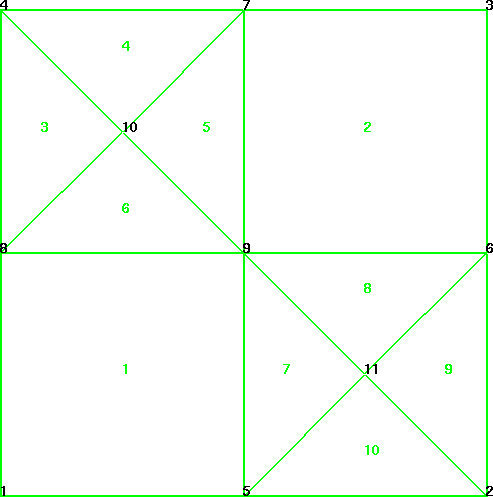
\includegraphics[width=.9\textwidth]{hybrid_mesh}}
  \caption{Hybrid element mesh (note that the numbers are off by one)}
\end{figure}

\end{document}
